Tunnistimme aineistostamme eri oppilastyyppejä.
Lähes kaikki kyselyyn vastanneet opiskelijat pitivät harjoituskurssia hyödyllisenä.
Syyt kuitenkin vaihtelivat; suuri osa ($n=9$) piti kurssia hyödyllisenä sen kertaavan luonteen vuoksi: ``Ainakin on jotain tullut kerrattua.'', ``Olen saanut kertausta''.
Neljän opiskelijan mielestä kurssilla on opittu myös uusia asioita, muun muassa laskimen käyttötaitoa: ``Olen saanut apua mm. laskimen käyttöön (alussa täysi painajainen) sek ekstra tehtävät ovat parantaneet laskutaitojani.''
Myös tekemällä oppimisen ja laskurutiinin kehittymisen merkitystä korostettiin: ``Täällä tulee tehtyä tehtäviä & ryhmä on pieni joten saa apua.'', ``Saanut lisää laskurutiinia ja oppinut lisää jo käytyjä asioita''. 
Kuusi opiskelijaa ei vastannut kysymykseen.
Hyvänä ominaisuutena pidettiin myös sitä, että apua ja neuvontaa on saatavilla: ``Olisi voinut olla enemmänkin, mutta olen kuitenkin voinut kysyä asioita, jotka tunneilta jäi epäselväksi.''

\begin{figure}[h!]
\centering
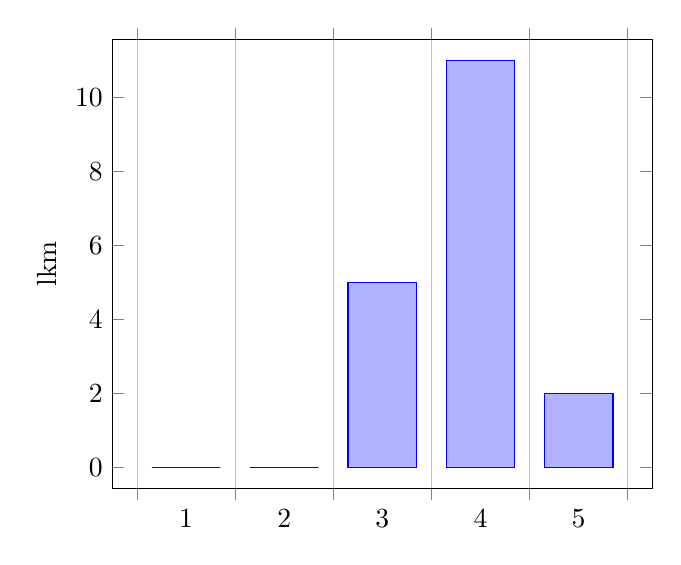
\begin{tikzpicture}
\begin{axis}[x tick label 
style={/pgf/number format/1000 sep=}, ylabel=lkm, enlargelimits=0.05, legend style={at={(0.5,-0.15)}, anchor=north,legend columns=-1},ybar interval=0.7]
\addplot coordinates {(1,0) (2,0) (3,5) (4,11) (5,2) (6,0)}; % miksei piirrä vikaa asiaa? :3
\end{axis}
\end{tikzpicture}
\caption{``Harjoituskurssista on ollut minulle hyötyä.''}
\end{figure}

\subsection{Kisälliopetus}
Kurssi toteuttaa kisälliopetuksen piirteet opiskelijoiden vastauksien mukaan hyvin.
Suurin osa opiskelijoista ($n=12$) kiitteli vastauksissaan sitä, että apua on saatavilla hyvin: ``On saanut aina apua, kun on tarvinnut.''
Loput ($n=7$) opiskelijat eivät kommentoineet vastausta, mutta olivat jokseenkin samaa mieltä tai täysin samaa mieltä siitä, että kurssilla saa apua hyvin.
Kysymyksen avoimeen perusteluosioon vastasi yheksän ($n=9$) opiskelijaa. Vastauksista kävi ilmi, että opiskelijat kokivat, että harjoituskurssilla saa paremmin apua tehtävien tekoon kuin tavallisella kurssilla, sillä ryhmä on pienempi, kaikki aika käytetään laskemiseen ja että paikalla on auskuja: ``Apua on aina tarjolla sitä tarvitseville varsinkin kun auskut ovat paikalla. Tämä avun saanti on suurin ero normikurssien ja matikka 15 välillä'', ``Pieni ryhmä on hyvä sillä opella on enemmän aikaa auttaa''.  Avun saamista tehtävien ratkaisemisessa kiiteltiin kurssin parhaimpana puolena: ``Suurin plussa! että saa pua''. 

Avoimeen kysymykseen ``Saatko sellaista apua, mitä kaipaat? Minkälaista apua kaipaat matematiikassa?'' kolmetoista ($n=13$) vastasi myöntävästi sekä kaipaavansa apua ja yksi vastasi, ettei kaipaa apua. Neljä opiskelijaa jätti vastaamatta kysymykseen. 

Myönteisissä vastauksissa esimerkiksi kaivattiin jotakuta selventämään kysymystä: ``Välillä on vaikea hahmottaa, mitä kysymys minulta haluaa joten opettajan läsnäolo ja tarvittaessa apu on helpottanut vaikeimpien tehtävien tekoa merkittävästi.'' , ``Kyllä lisää selitystä kaivataan''. Vaikeissa ja soveltavissa tehtävissä kaivattiin apua: ``Kyllä, tarvitsen apua joihinkin vaikeisiin tehtäviin'', Saan hyvin apua. Usein kaipaa apua vaikeimpiin sovelluksiin.''. 

Opettajan osuutta kiiteltiin, erityisesti sitä, että opettaja osaa neuvoa silloinkin, kun ei itsekään tiedä mitä kysyisi: ``Yleensä en osaa sanoa millaista apua kaipaan, mutta Päivi osaa aina neuvoa :)''. Myös laskimen käytössä kaivattiin ja oli saatu apua kurssilla. 

\begin{figure}[h!]
\centering
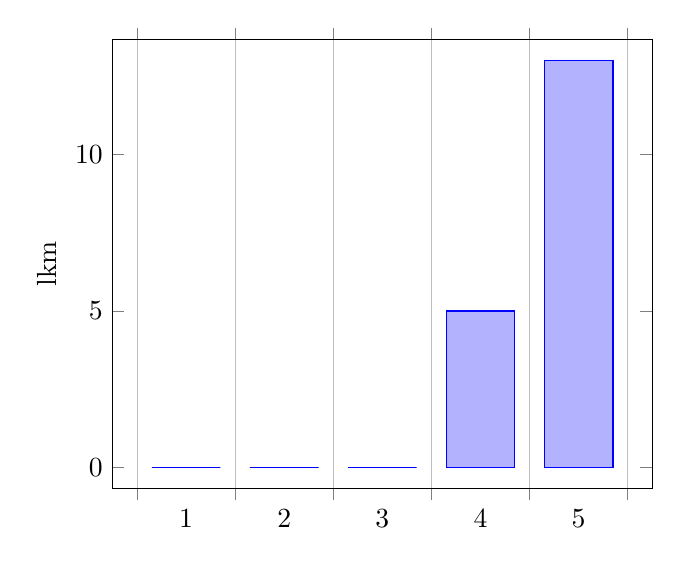
\begin{tikzpicture}
\begin{axis}[x tick label 
style={/pgf/number format/1000 sep=}, ylabel=lkm, enlargelimits=0.05, legend style={at={(0.5,-0.15)}, anchor=north,legend columns=-1},ybar interval=0.7]
\addplot coordinates {(1,0) (2,0) (3,0) (4,5) (5,13) (6,0)}; % miksei piirrä vikaa asiaa? :3
\end{axis}
\end{tikzpicture}
\caption{``Saan harjoituskurssilla apua tehtävien ratkaisemiseen.''}
\end{figure}

Myös \emph{scaffolding}-ilmiö esiintyy vastauksissa.

\begin{figure}[h!]
\centering
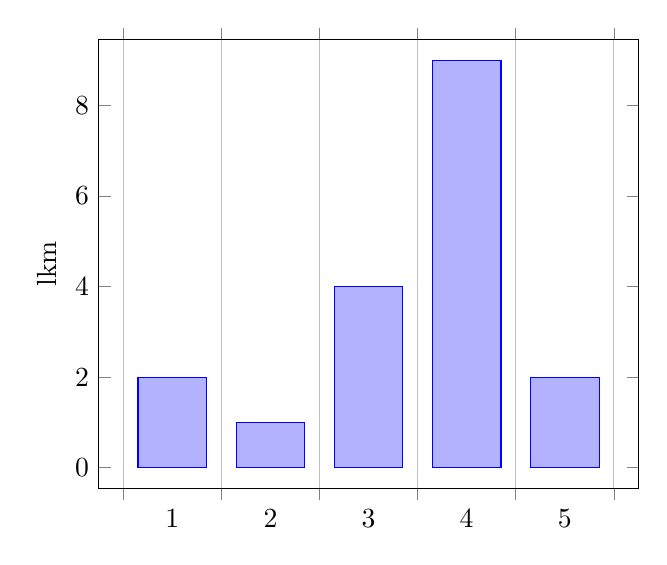
\begin{tikzpicture}
\begin{axis}[x tick label 
style={/pgf/number format/1000 sep=}, ylabel=lkm, enlargelimits=0.05, legend style={at={(0.5,-0.15)}, anchor=north,legend columns=-1},ybar interval=0.7]
\addplot coordinates {(1,2) (2,1) (3,4) (4,9) (5,2) (6,0)}; % miksei piirrä vikaa asiaa? :3
\end{axis}
\end{tikzpicture}
\caption{``Saan harjoituskurssilla tehtyä sellaisiakin tehtäviä, joita en itsenäisesti osaisi tehdä.''}
\end{figure}

Itsevarmuus omasta osaamisesta vaikuttaa opiskelijan matematiikkapelkoon.
Se, että opiskelija kokee korkeaa minäpystyvyyden tunnetta on myös välttämätöntä \emph{flow}-tilaan pääsemiseksi.
%Vastauksista voi myös päätellä, että harjoituskurssi torjuu opiskelijoiden matematiikkapelkoa.

\begin{figure}[h!]
\centering
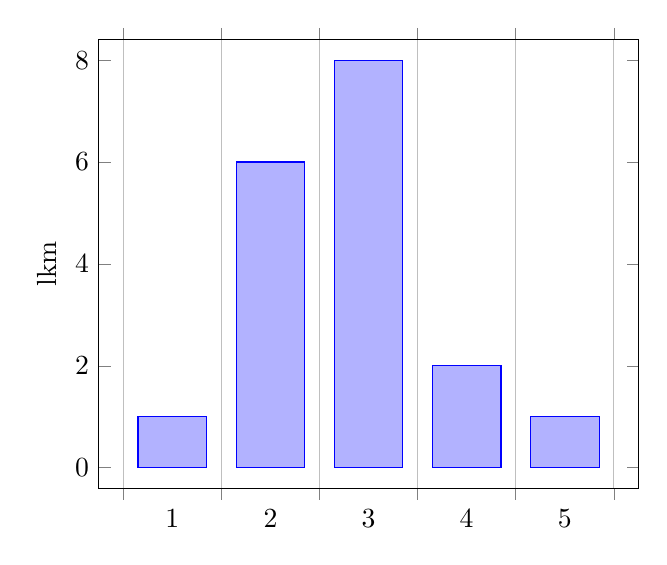
\begin{tikzpicture}
\begin{axis}[x tick label 
style={/pgf/number format/1000 sep=}, ylabel=lkm, enlargelimits=0.05, legend style={at={(0.5,-0.15)}, anchor=north,legend columns=-1},ybar interval=0.7]
\addplot coordinates {(1,1) (2,6) (3,8) (4,2) (5,1) (6,0)};
\end{axis}
\end{tikzpicture}
\caption{``Harjoituskurssi on lisännyt itsevarmuuttani matematiikan osaamisen suhteen.''}
\end{figure}

Opiskelijat, jotka olivat täysin tai jokseenkin eri mieltä väitteen kanssa vastasivat muun muassa, että itsevarmuus riippuu vain käsiteltävien aiheiden mielekkyydestä, että yksi kurssi ei riitä itsevarmuuden kehittämiseen ja että itsevarmuutta vähentää se, että ei saa helpoksi luonnehdittua tehtävää ratkaistua. 

On mielenkiintoista, että menestys matematiikan kursseilla ei välttämättä paranna itsetuntoa matematiikan osaamiseen suhteen. Vastauksista ilmeni esimerkiksi, että vaikka opiskelija koki harjoituskurssin parantaneen hänen menestystään muillakin matematiikan kursseilla, niin hän edelleen koki matematiikan vaikeaksi ja etenemistahdin liian nopeaksi. Yleisesti ottaen kuitenkin ne, joiden mielestä kurssi oli parantanut heidän menestystään, kokivat, että se oli myös lisännyt heidän itsevarmuuttaan, ja päin vastoin.

Opiskelijat, jotka oli samaa tai täysin samaa mieltä perustelivat vastaustaan esimerkiksi siten, että laskemisen määrän koettiin edistävän oppimista ja lisäävän itsetuntoa: ``Lasken enemmän ja saan apua -> edistyn'', ``Harjoitus tekee mestarin''. 



\subsection{Opiskelijoiden matematiikkakuva}
Kyselyvastauksista kävi ilmi, että moni opiskelija pitää matematiikkaa enimmäkseen laskemisena.
Lisäksi matemaattisen taidon koetaan kehittyvän harjoittelun avulla.

\subsection{Viihtyvyys kurssilla}
Opiskelijoiden mielestä harjoituskurssilla oli pääosin mukavaa. Ainoastaan kaksi opiskelijaa oli väitteen ``Harjoituskurssilla on mukavaa'' kanssa eri mieltä, ja perustelivat vastauksiaan kurssin tylsyydellä ja laskemisen puuduttavuudella. Yksi opiskelija ei ollut samaa eikä eri mieltä. Muut viisitoista ($n=15$) olivat joko samaa tai täysin samaa mieltä siitä, että kurssilla on mukavaa. Vastauksissa nousi positiivisena esille rento, ei-koulumainen ilmapiiri kurssilla, mahdollisuus jutella kavereiden kanssa, ratkoa tehtäviä yhdessä ja syödä laskemisen lomassa. Opiskelijat kokivat myös, että suhde opettajaan oli harjoituskurssilla välittömämpi. 

Toisaalta vapaus kurssilla koettiin myös ongelmaksi; eräs opiskelija reflektoi omaa panostaan kurssilla seuraavasti: ``Kurssilla on hyvä tunnelma ja vapaampaa puhua kavereiden kanssa. Tämä toisaalta on myös ongelma ja mietinkin joskus että puhua voisi vapaa-ajallakin ja että onko kurssi turha minulle''



\subsection{Kurssin vaativuustaso}
Osalle opiskelijoista kurssi oli sopivan vaativa, mutta monet kokivat myös tylsistyvänsä tunnilla.
Tämä tarjoaisi hedelmällisen mahdollisuuden eriyttää opetusta; jos tehtävämonisteita olisi kaksi, kertaava ja syventävä, kurssi palvelisi laajempaa opiskelijajoukkoa.
Koska kurssisuoritukseen riittää vain läsnäolo, valmistaa kurssi myös korkeakoulujen akateemiseen vapauteen; opiskelijalla on vastuu omasta työskentelystään.
Tämä saattaa lisäksi hillitä matematiikkapelkoa, sillä opiskelijalla ei ole paineita suorittaa tiettyä määrää tehtävistä.

\subsection{Miten kurssia voisi kehittää?}
Opiskelijoiden vastauksista ei noussut mitään yhtä erityistä kehitysideaa, vaan ideoita oli vaihtelevasti. Kahdeksan ($n=8$) opiskelijaa jätti vastaamatta kysymykseen ja kolme ($n=3$) vastasi ``en tiedä''. Lopuissa vastauksissa toivottiin jotkin muuta ajankohtaa kurssille, lisää opettajia tai ohjaajia, hauskempia ja pohtimista vaativia tehtäviä, opittujen asioiden syventämistä. Myös toivottiin, että tehtyjen tehtävien määrälle asetettaisiin jokin vähimmäisraja, jotta se motivoisi tekemään tehtäviä. Yksi opiskelija vastasi, että kurssi on ollut hyvä näin. 



